\subsection{Fly exposure policy}
The policy is triggered by the temperature. If the temperature is above 20, the policy goes in effect. This temperature is based on the findings by \cite{schou_temperature_2013}. It assumes an immediate reduce of 20\% on the rate of human exposure to infectious flies.

\subsubsection{Policies in the base model}
\textcolor{red}{Move this text to the appendix - iterative approach to developing the policies}
A policy regarding slaughtering was modeled into the base model, which will be tested under the same scenarios as the base model. The food safety and handling policy, also dubbed the Safe Slaughtering policy, goes into effect when Cost of Illness reaches a certain threshold, set at a 100 million euros. This policy means that the rate of cross-contamination drops by 20\%.  

\begin{figure}[h!]
    \centering
    \begin{minipage}{0.45\textwidth}
        \centering
        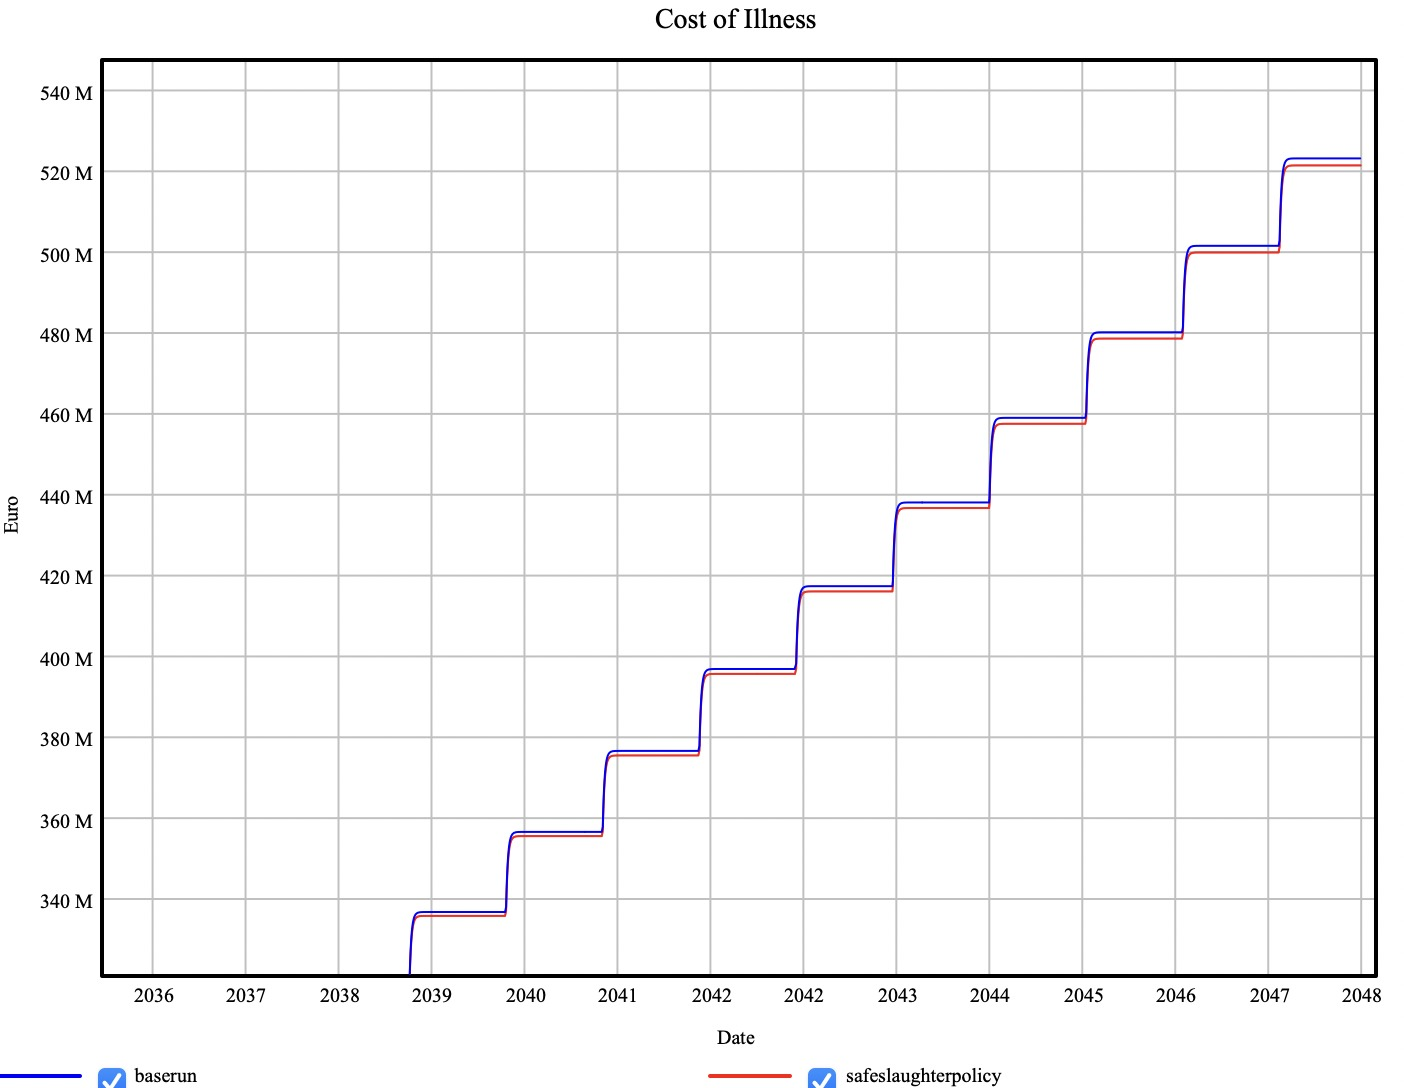
\includegraphics[width=1\textwidth]{images/p_coi.jpeg} 
        \caption{Cost of Illness in the Safe Slaughtering base run}
        \label{fig:p_coi}
    \end{minipage}\hfill
    \begin{minipage}{0.45\textwidth}
        \centering
        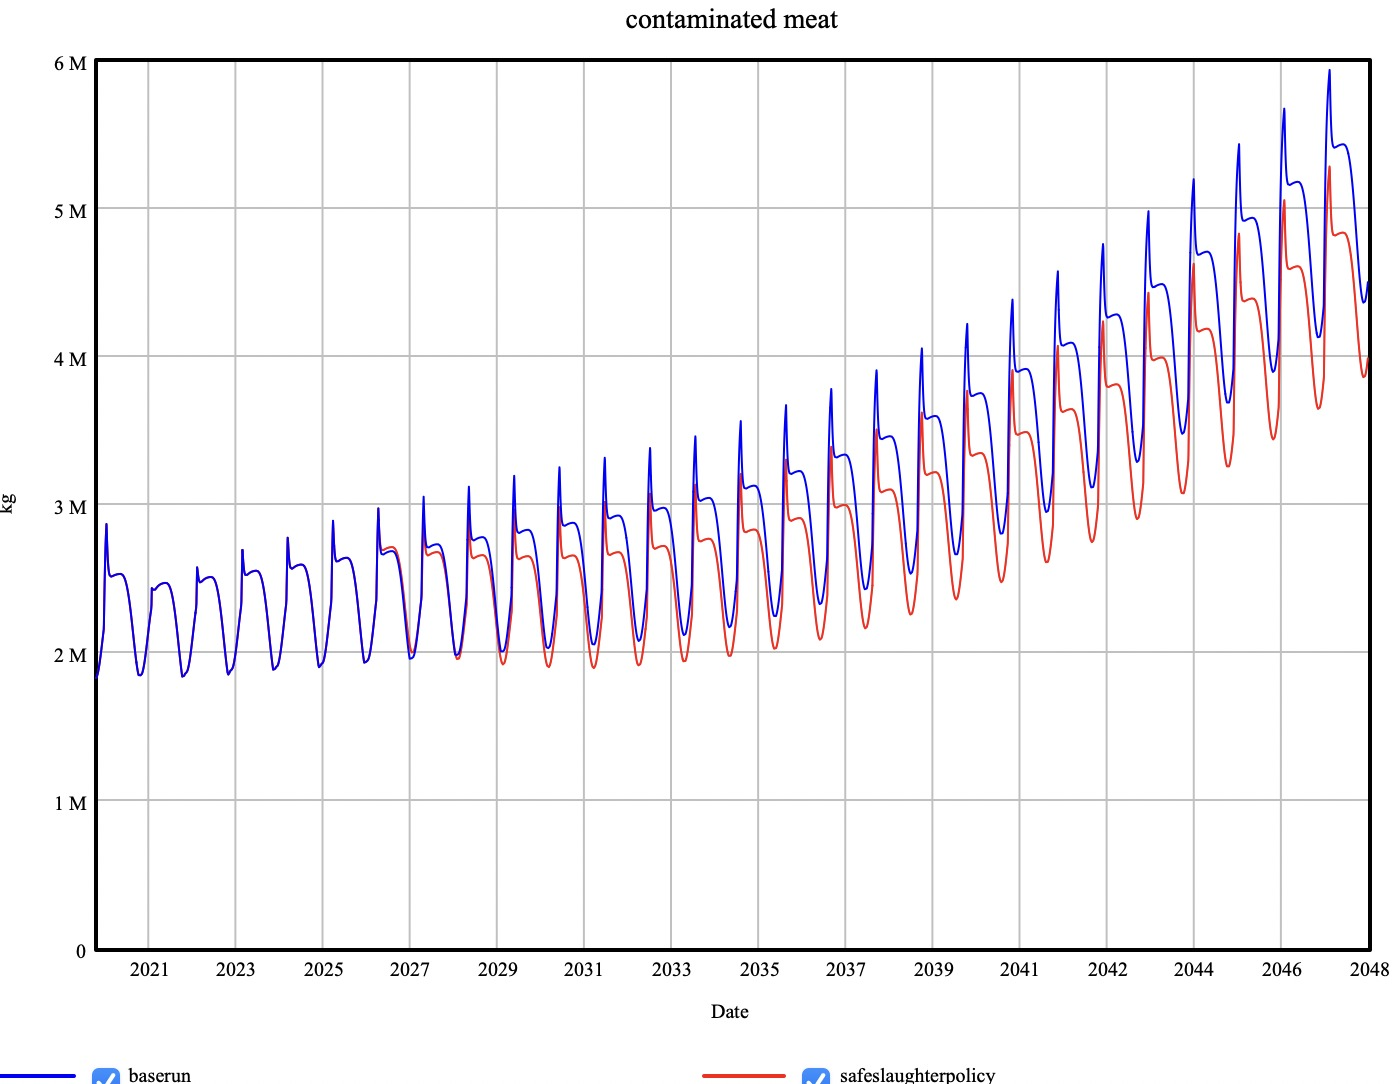
\includegraphics[width=1\textwidth]{images/p_meat.jpeg}
        \caption{Contaminated chicken meat in the Safe Slaughtering base run}
        \label{fig:p_meat}
    \end{minipage}
\end{figure} 

Model behaviour under this policy is reasonable. Once the food safety and handling policy goes into effect, the stock of contaminated meat decreases before slowly increasing again. This shows that it has an immediate effect, which stays over time but then continues growing. 

The odd spikes in Figure \ref{fig:p_meat} are similar to the ones as explained in section \ref{s:b_base}. 

Another policy implemented was the campaign to limit human exposure to flies, dubbed the No Fly Zone. This campaign would inform the Dutch population on how to minimize attractive environments for fly propagation. This policy reduces the rate of human exposure to infectious flies by 20\%. 

\begin{figure}[h!]
    \centering
    \begin{minipage}{0.45\textwidth}
        \centering
        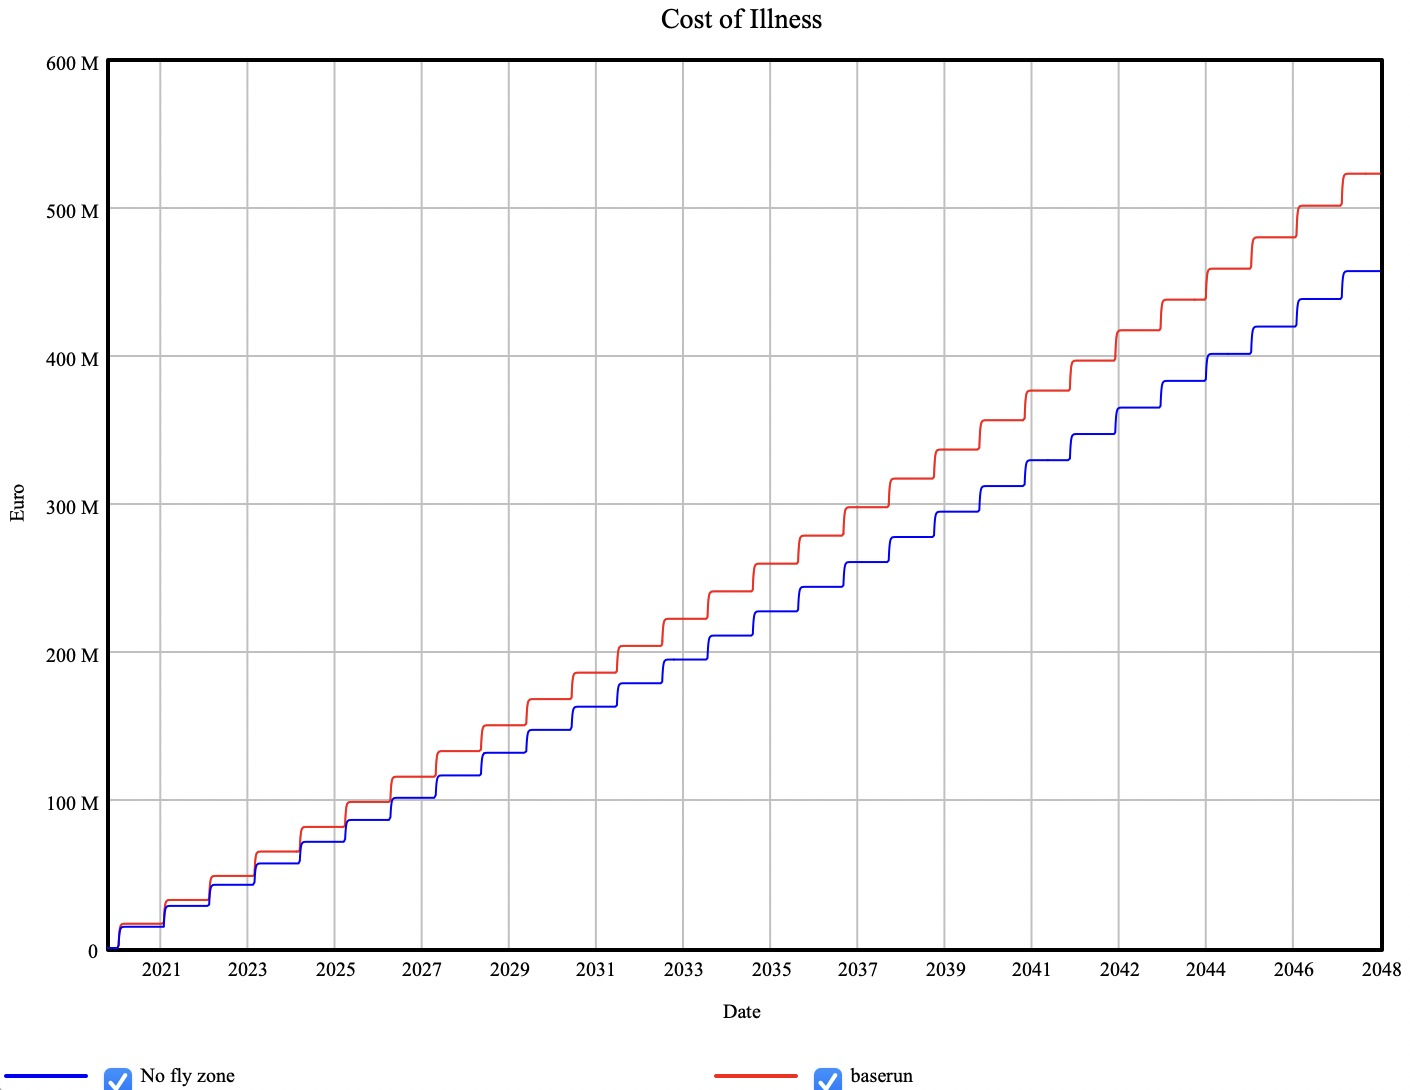
\includegraphics[width=1\textwidth]{images/p2_coi.jpeg} 
        \caption{Cost of Illness in the No Fly Zone base run}
        \label{fig:p2_coi}
    \end{minipage}\hfill
    \begin{minipage}{0.45\textwidth}
        \centering
        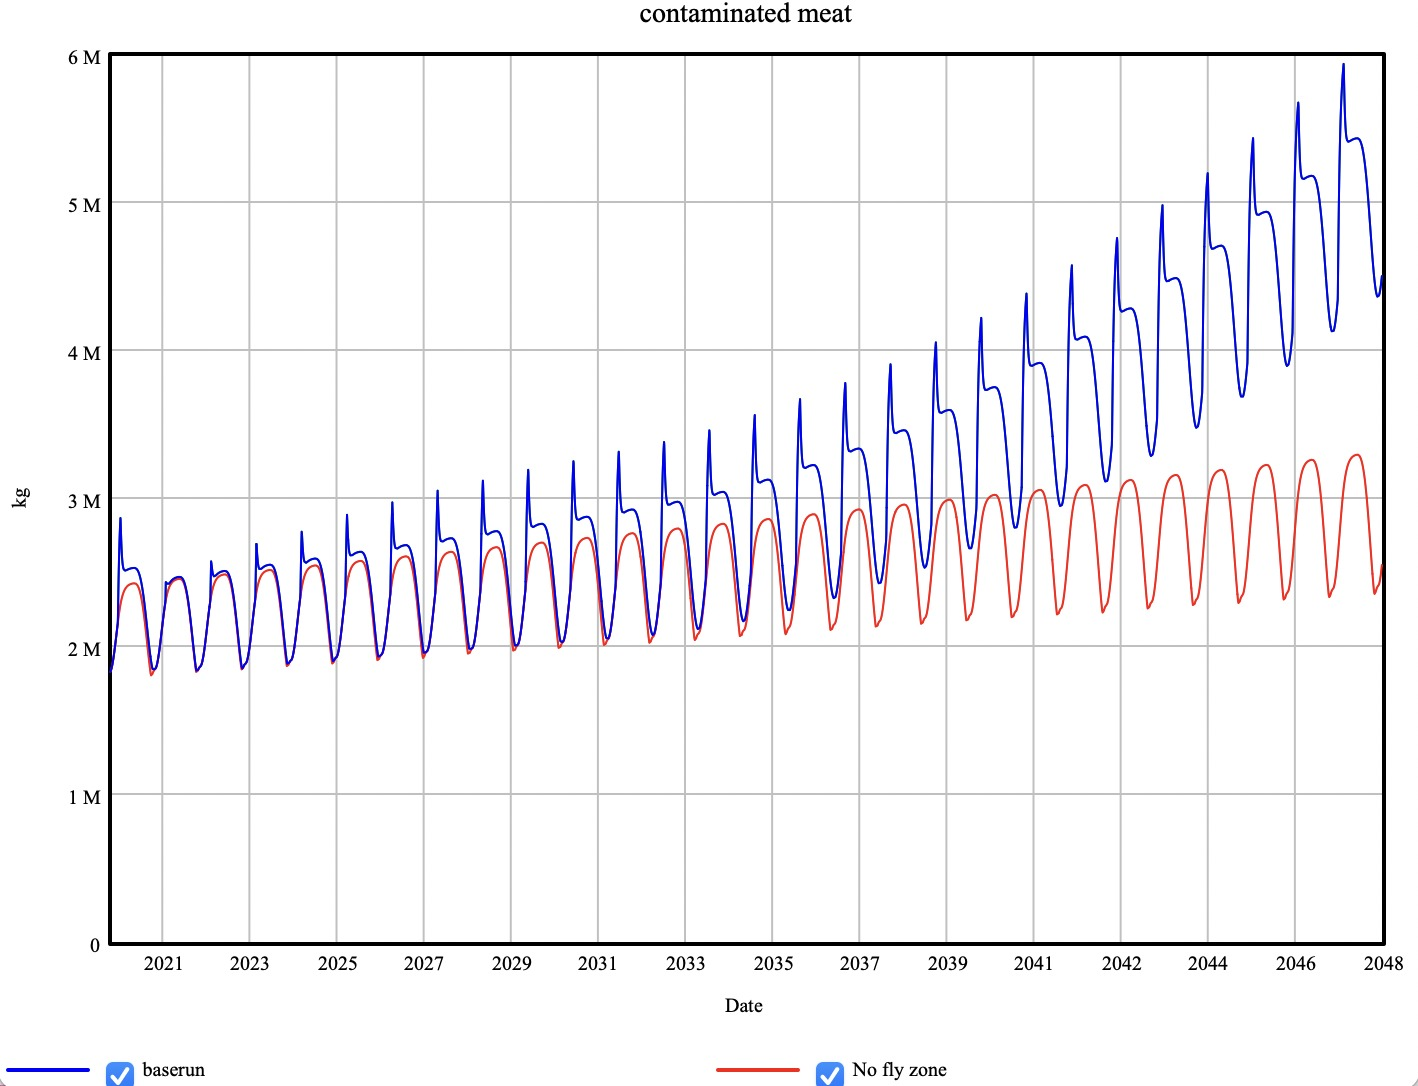
\includegraphics[width=1\textwidth]{images/p2_meat.jpeg}
        \caption{Contaminated chicken meat in the No Fly Zone base run}
        \label{fig:p2_meat}
    \end{minipage}
\end{figure} 

\begin{figure}[h]
\centering
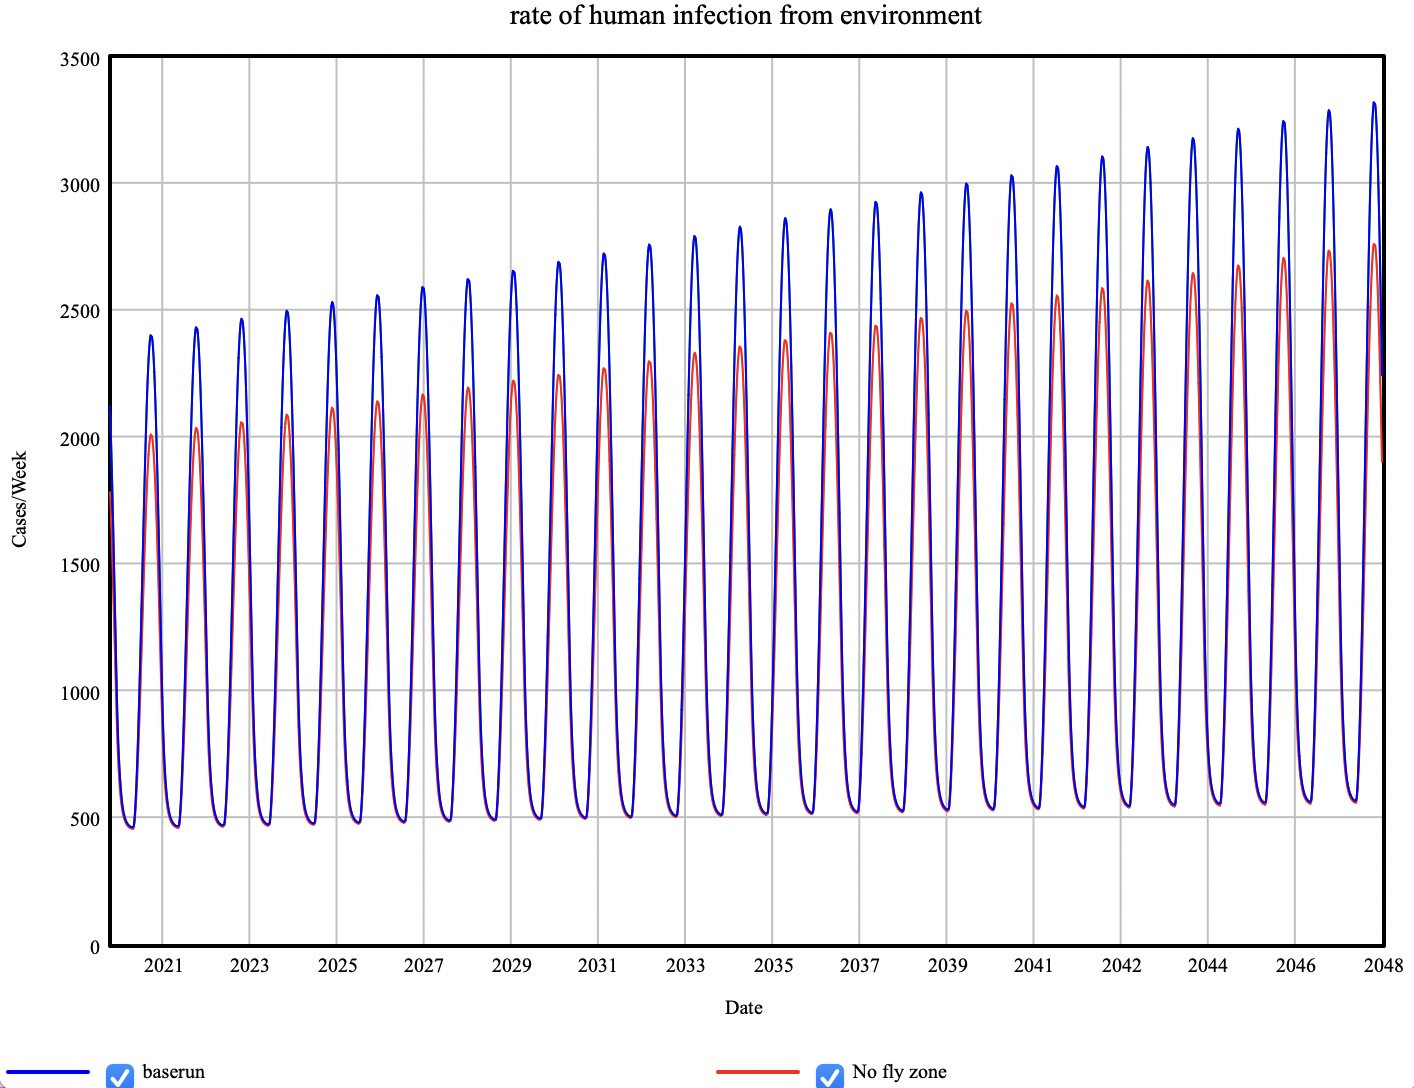
\includegraphics[width=0.45\textwidth]{images/p2_humanenvo.jpeg}
\caption{Human infections from the environment in the No Fly Zone base run }
\label{fig:p2_humanenvo}
\end{figure}

It can be seen in Figure \ref{fig:p2_meat} that the policy removes the strange peaks in the baserun. This is most likely due to the fact that the policy lowers the number of \textit{Campylobacter} cases, which mitigates the decrease of chicken meat consumption. This means that the threshold isn't met to trigger the meat consumption behaviour while the stock of contaminated meat decreases accordingly. 

Another fly related policy which was implemented is the the Pest Control policy. This Pest Control policy entails a policy that target the infectious flies and attempts to exterminate these fly populations in areas they would most likely be found, such as slaughterhouses and chicken farms.  

\begin{figure}[h!]
    \centering
    \begin{minipage}{0.45\textwidth}
        \centering
        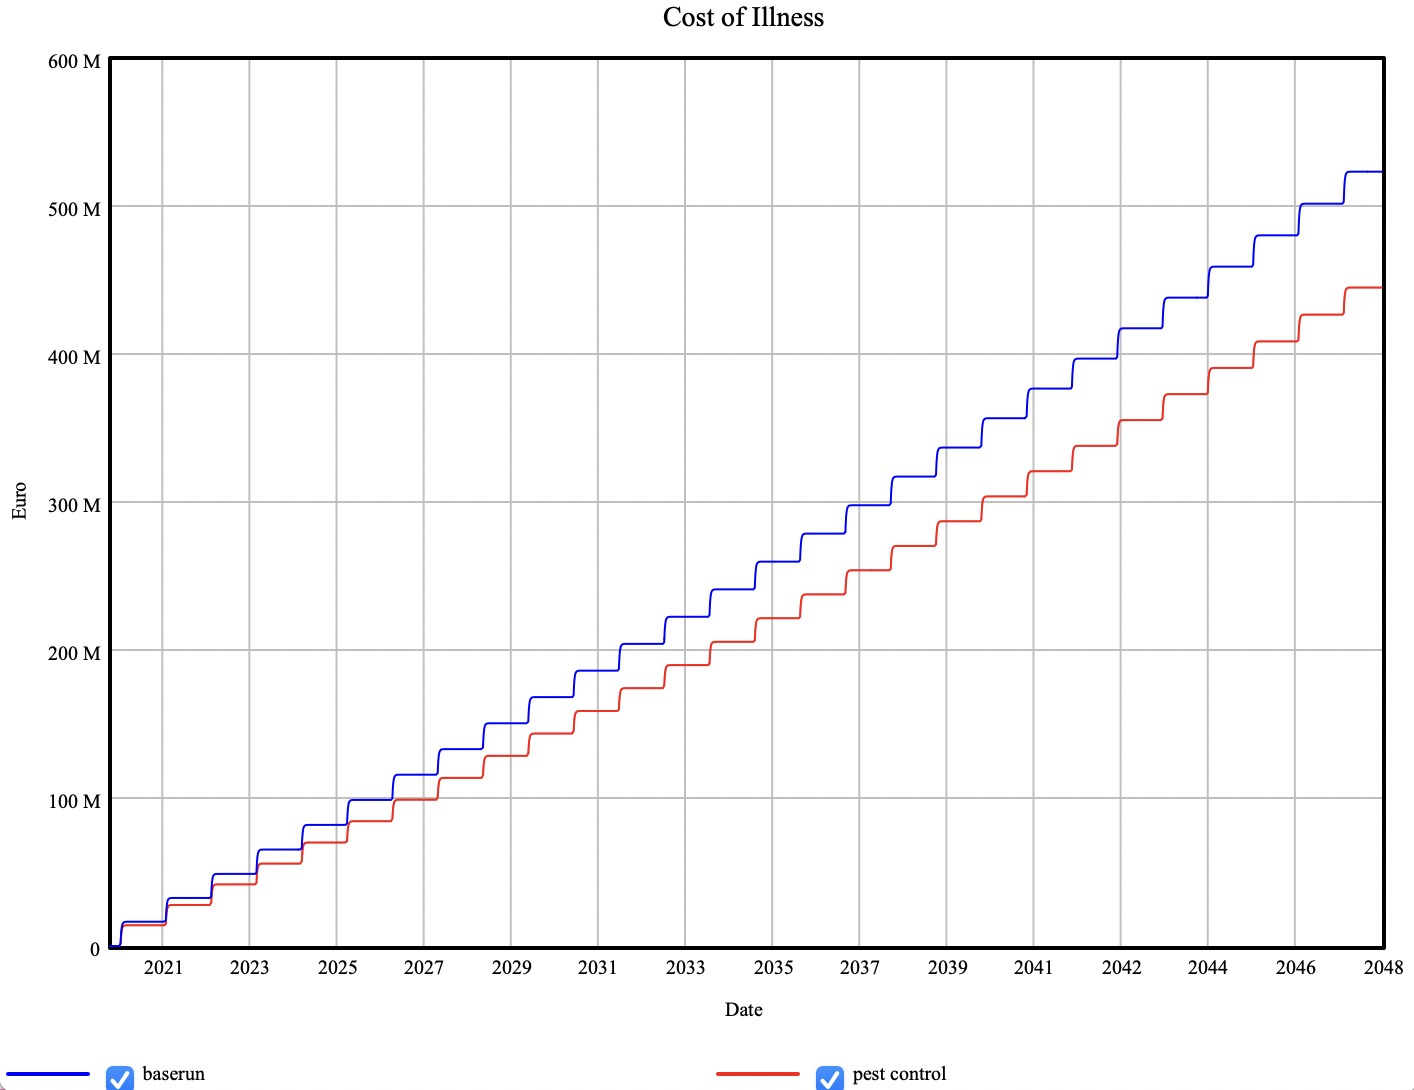
\includegraphics[width=1\textwidth]{images/p3_coi.jpeg} 
        \caption{Cost of Illness in the No Fly Zone base run}
        \label{fig:p3_coi}
    \end{minipage}\hfill
    \begin{minipage}{0.45\textwidth}
        \centering
        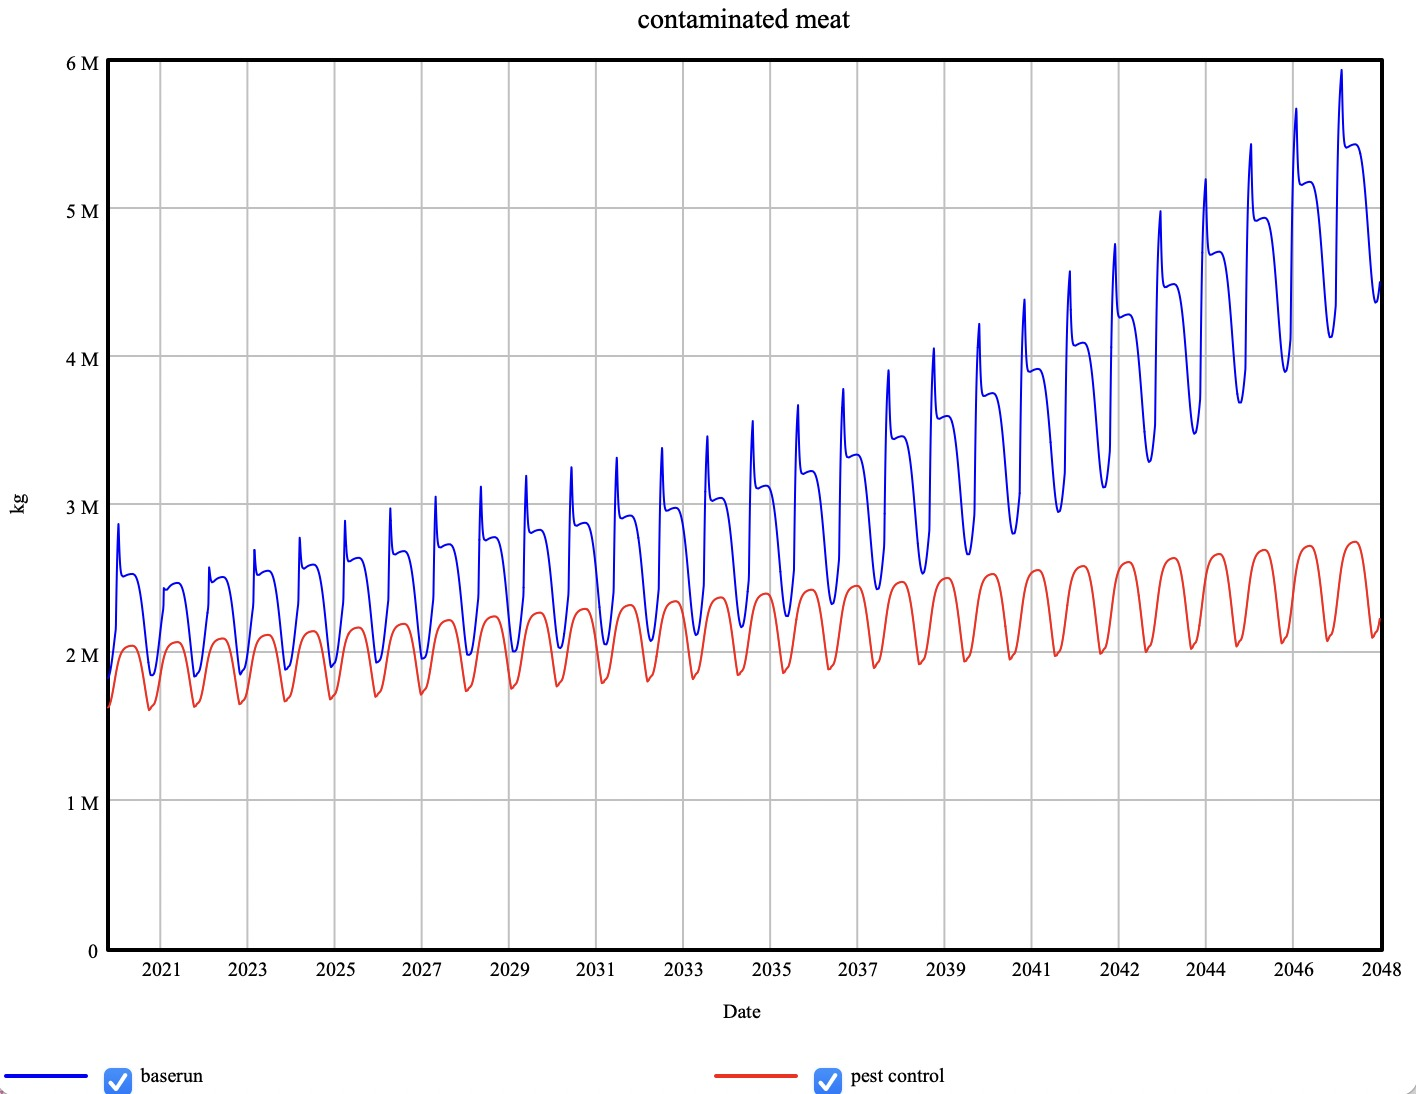
\includegraphics[width=1\textwidth]{images/p3_meat.jpeg}
        \caption{Contaminated chicken meat in the No Fly Zone base run}
        \label{fig:p3_meat}
    \end{minipage}
\end{figure} 

\begin{figure}[h!]
    \centering
    \begin{minipage}{0.45\textwidth}
        \centering
        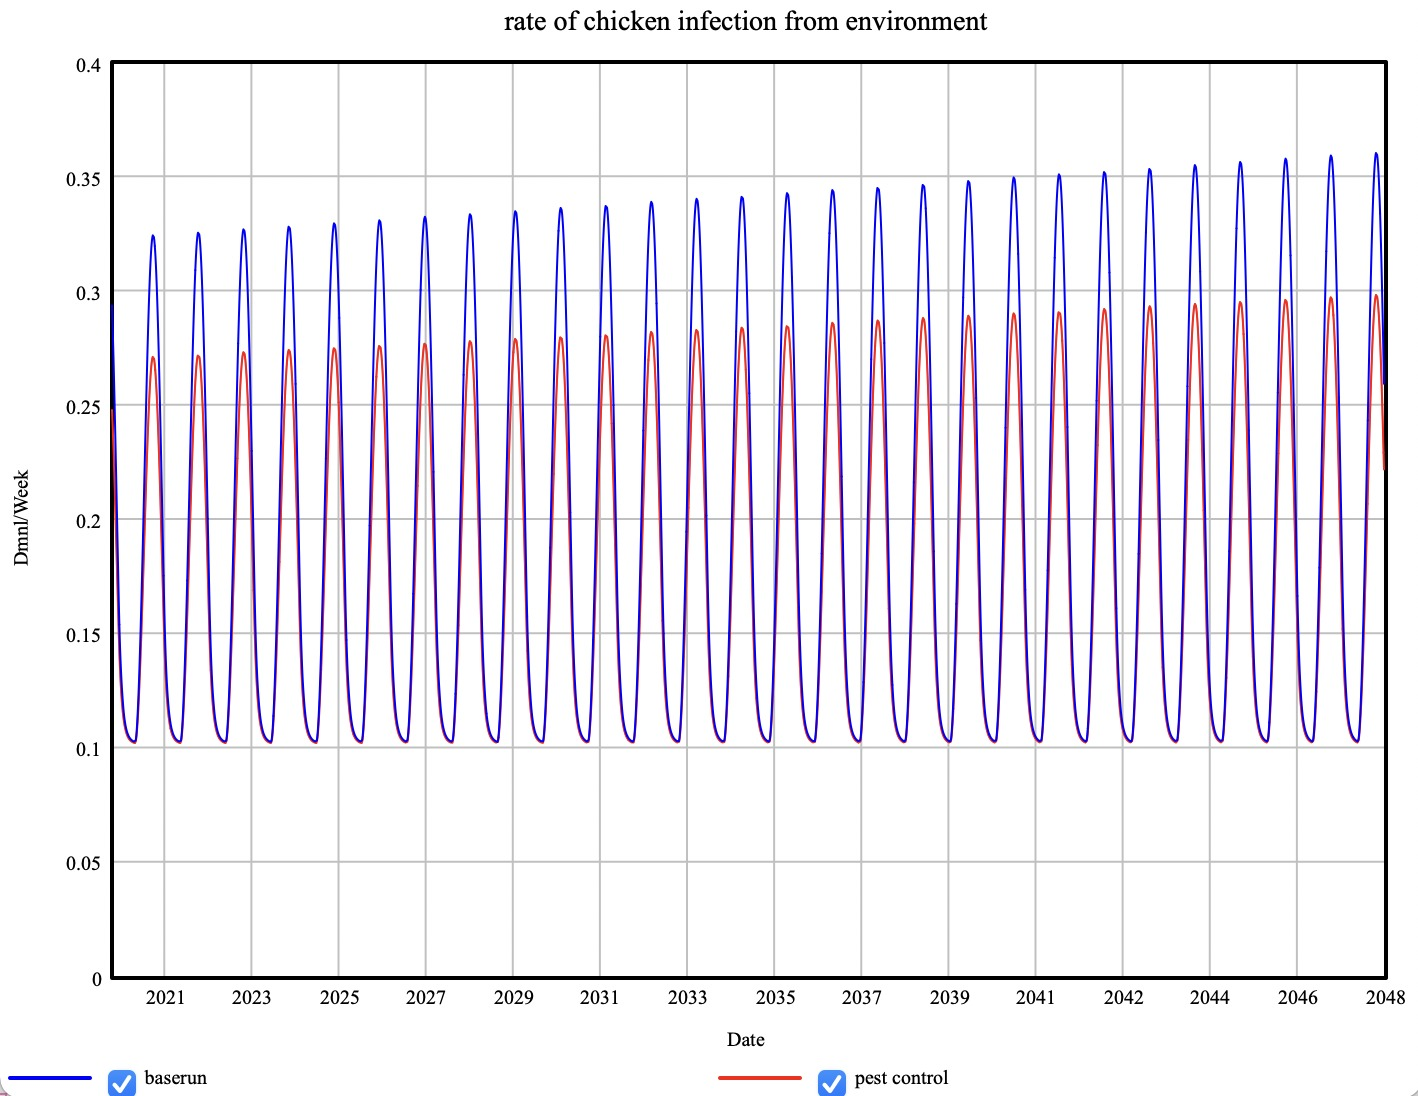
\includegraphics[width=1\textwidth]{images/p3_chicken.jpeg} 
        \caption{Chicken infections from the environment in the Pest Control base run}
        \label{fig:p3_chicken}
    \end{minipage}\hfill
    \begin{minipage}{0.45\textwidth}
        \centering
        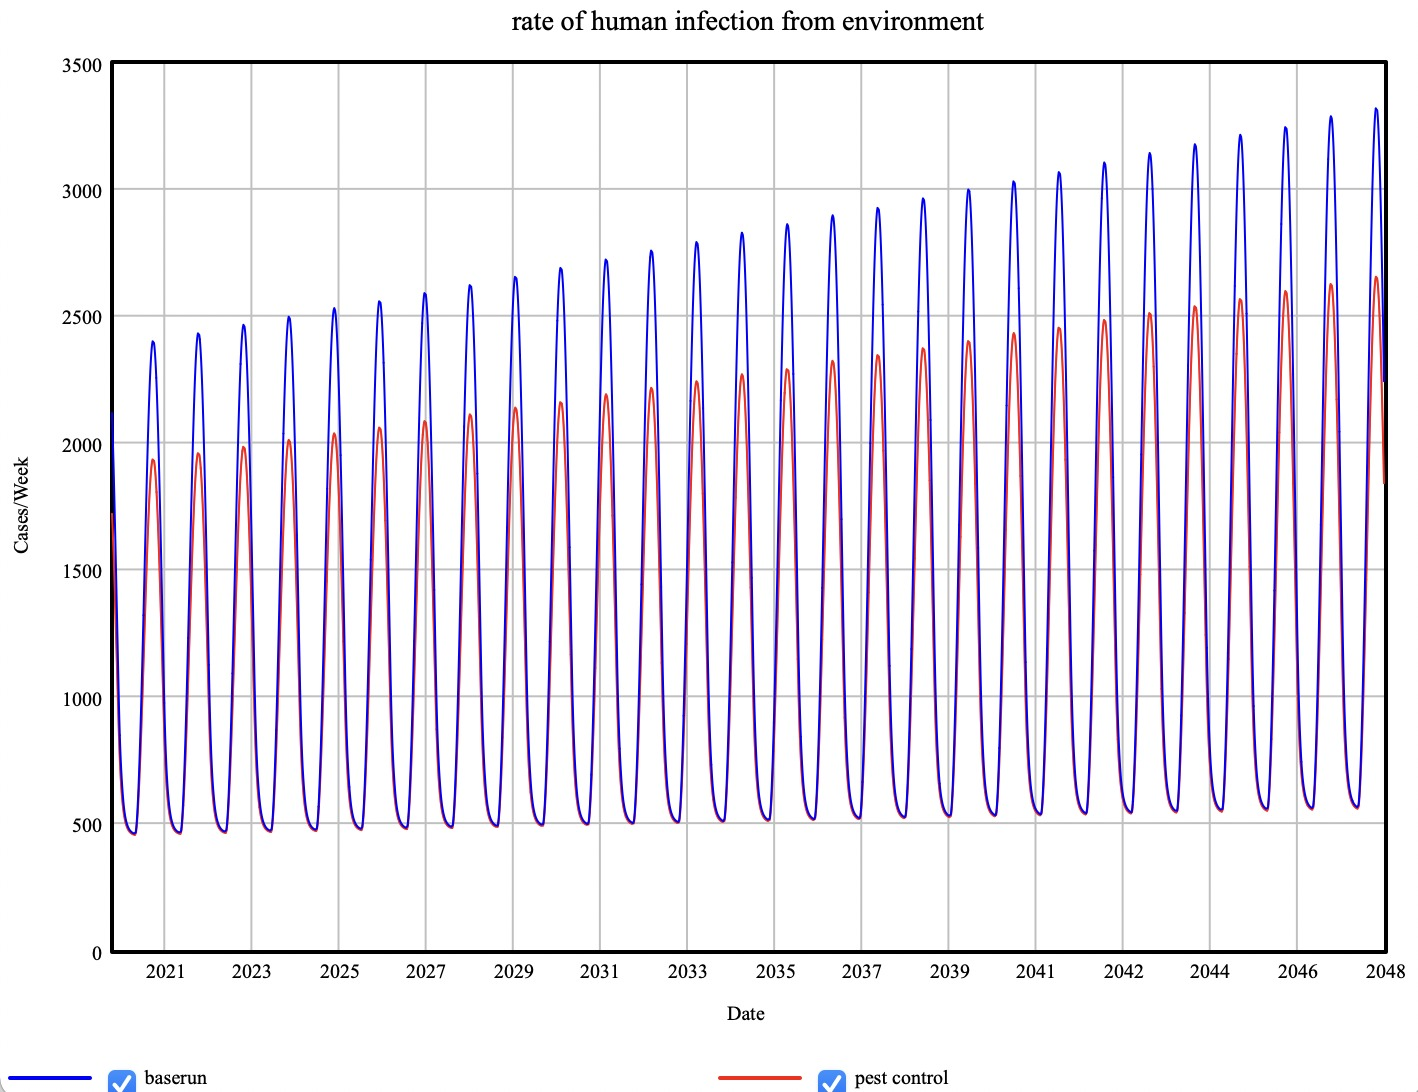
\includegraphics[width=1\textwidth]{images/p3_human.jpeg}
        \caption{Human infections from the environment in the Pest Control base run}
        \label{fig:p3_human}
    \end{minipage}
\end{figure} 

Two more policies regarding food were implemented, named food behaviour and preparation policies. Similar to the Safe Slaughtering policy, these policies go into effect when Cost of Illness reaches the 100 million threshold. These policies act on
\textit{consumption rate per person} and \textit{infections per kg of meat} respectively, by reducing these by 20\%.  

\begin{figure}[h!]
    \centering
    \begin{minipage}{0.45\textwidth}
        \centering
        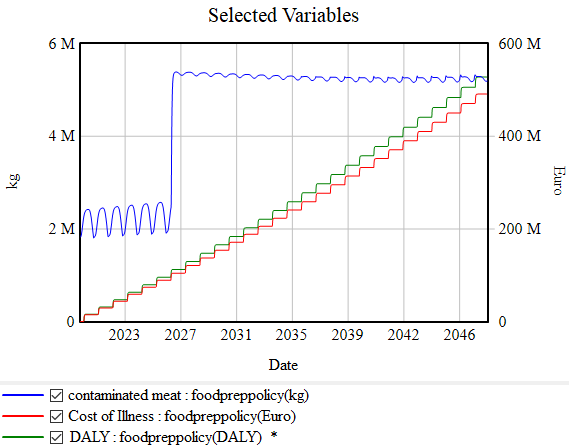
\includegraphics[width=1\textwidth]{images/foodbehaviourpolicy.png} 
        \caption{KPIs under food behaviour policy}
        \label{fig:foodbehav}
    \end{minipage}\hfill
    \begin{minipage}{0.45\textwidth}
        \centering
        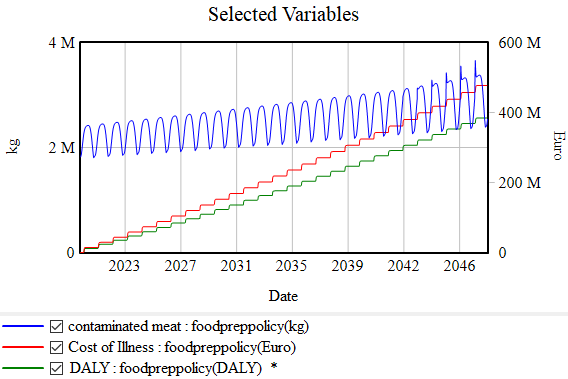
\includegraphics[width=1\textwidth]{images/foodpreparationpolicy.png}
        \caption{KPIs under food preparation policy}
        \label{fig:foodprep}
    \end{minipage}
\end{figure}
